\documentclass[12pt]{article}

% fonts

\usepackage[T1]{fontenc}
\usepackage{newtxtext}
\usepackage{bm}
\usepackage{amsthm} % before newtxmath b/c latex
\usepackage{newtxmath}
% \usepackage[bb=boondox,cal=cm]{mathalpha}
\usepackage{cancel}
\usepackage{amsmath}
\usepackage{amsfonts}
\usepackage{thmtools}
\usepackage{mathtools}
\usepackage{mathrsfs}
\usepackage{hyperref}
\usepackage{wrapfig}
% spacing

\usepackage[parfill]{parskip}
\setlength{\parindent}{0pt}
\setlength{\parskip}{2ex plus 0.2ex minus 0.2ex}

% geometry of the page

\usepackage[
paper  = letterpaper,
left   = 1in,
right  = 1in,
top    = 1in,
bottom = 1in,
]{geometry}

% references

\usepackage{natbib}


\begin{document}

\begin{flushleft}
\textbf{PSET 3 APMA4302} \\
Fred Angelo Garcia (fbg2107) \\
\today
\end{flushleft}

\vspace{0.1in}

We know the nonlinear reaction-diffusion equation
\begin{equation}
- \nabla^2 + \gamma u^p = f
\end{equation}
where $\gamma$ is a positive constant and $p>1$ is an integer. Using Dirichlet boundary conditions, the righthand side $f(x,y)$ is determined by the manufactured solutions, assuming the exact solution is given by
\begin{equation}
    u_{\rm exact}(x,y) = A \exp\left[-\frac{(x-x_0)^2 + (y-y_0)^2}{\sigma^2}\right]
\end{equation}
where -- the problem tells us -- $(x_0, y_0)$ is a point in the unit square, $\sigma$ is a positive constant controlling the width of the Gaussian with amplitude $A$.

WE are given the code \texttt{poisson2d.c}, which solves the linear version ($\gamma = 0$) as a discrete problem
\begin{equation}
A \mathbf{x} = \mathbf{b}.
\end{equation}

To help setup some intuition, Ch4 of Bueler says it balances the defussion term $-\nabla^2 u$ with the reaction term $\gamma u^p$ and the source term $f$ for a substance with concentration $u$ that is diffusing, reacting, and being produced. 



\section{Question 1}

We can write the nonlinear problem as a system of equations in the form of $F(\mathbf{u}) = 0$ using finite differences to discritize the Laplacian. We can then solve this system using Newton's method, which requires us to compute the Jacobian.

On an $N-$point grid, with spacing $h_x= 1 / (N-1)$ and similarly $h_y$ where $x_j = j h_x$ for $j = 1, \ldots, N-1$ and $y_k = k h_y$ for $k = 1, \ldots, N-1$.

We begin (following eq. 4.14 but for two dimensions) by writing the finite difference approximation to the Laplacian as
\begin{equation}
    -\nabla^{2}u\approx-\frac{u_{i+1,j}-2u_{i,j}+u_{i-1,j}}{h_{x}^{2}}-\frac{u_{i,j+1}-2u_{i,j}+u_{i,j-1}}{h_{y}^{2}},
\end{equation}
which gives us the discritized version of the PDE as
\begin{equation}
    F_{i,j}(\mathbf{u})=-\frac{u_{i+1,j}-2u_{i,j}+u_{i-1,j}}{h_{x}^{2}}-\frac{u_{i,j+1}-2u_{i,j}+u_{i,j-1}}{h_{y}^{2}}+\gamma u_{i,j}^p-f_{i,j} = 0.
\end{equation}
Given that we are  in a unit square, we can set $h_x = h_y = h$ we can massage the equations to being
\begin{equation}
    F_{i,j}(\mathbf{u})=-\frac{u_{i+1,j}+u_{i-1,j}+u_{i,j+1}+u_{i,j-1}-4u_{i,j}}{h^{2}}+\gamma u_{i,j}^p-f_{i,j} = 0
    \label{eq:discretized}
\end{equation}
with the Dirichlet boundary conditions $u(x_i, y_j) = u_{\rm exact}(x_i, y_j)$, giving us the auxiliary equations
\begin{equation}
    F_{i,j}(\mathbf{u}) = u_{i,j} - u_{\rm exact}(x_i, y_j) = 0
    \label{eq:boundary}
\end{equation}
for $i = 0, N-1$ and $j = 0, N-1$. In short, the interior nodes are determines by Eq. \ref{eq:discretized} and the boundary nodes are determined by Eq. \ref{eq:boundary}.

\section{Question 2}
We alos need the elemens of the Jacobian matrix $J_{i,j}(\mathbf{u}) = \partial F_i / \partial u_j$.

For the boundary nodes, we have
\begin{equation}
    J_{i,j}(\mathbf{u}) = \frac{\partial F_{i,j}(\mathbf{u})}{\partial u_{i,j}} = 1 \quad \text{for } i = 0, N-1 \text{ and } j = 0, N-1
\end{equation}
and all other entries are zero. The function $F_{i,j}$ depends on five unknowns $u_{i,j}$, $u_{i+1,j}$, $u_{i-1,j}$, $u_{i,j+1}$, and $u_{i,j-1}$, which forms the five-point stencil. 
\begin{equation}
\dfrac{\partial F_{i,j}(\mathbf{u})}{\partial u_{i,j}} = 2 \left(\frac{h_y}{h_x} + \frac{h_x}{h_y}\right) + h_x h_y \gamma p u_{i,j}^{p-1} 
\end{equation}
along with $$\dfrac{\partial F_{i,j}(\mathbf{u})}{\partial u_{i+1,j}} = \dfrac{\partial F_{i,j}(\mathbf{u})}{\partial u_{i-1,j}} = -\frac{h_y}{h_x}$$ and $$\dfrac{\partial F_{i,j}(\mathbf{u})}{\partial u_{i,j+1}} = \dfrac{\partial F_{i,j}(\mathbf{u})}{\partial u_{i,j-1}} = -\frac{h_x}{h_y}.$$ Or given that $h_x = h_y = h$, we have
\begin{equation}
    \dfrac{\partial F_{i,j}(\mathbf{u})}{\partial u_{i,j}} = 4 + h^2 \gamma p u_{i,j}^{p-1}
\end{equation}
and $$\dfrac{\partial F_{i,j}(\mathbf{u})}{\partial u_{i+1,j}} = \dfrac{\partial F_{i,j}(\mathbf{u})}{\partial u_{i-1,j}} = \dfrac{\partial F_{i,j}(\mathbf{u})}{\partial u_{i,j+1}} = \dfrac{\partial F_{i,j}(\mathbf{u})}{\partial u_{i,j-1}} = -1.$$

\section{Question 3}
We will use the rection setup which solves the 1D nonlinear reaction-diffusiuon equation with linear reaction term $R(u)= -\rho\sqrt{u}$ to make it into 2D and instead use the reaction term $R(u) = \gamma u^p$.

Please see \texttt{reaction2d.c} for the code implementation, which is based on \texttt{poisson2d.c} and \texttt{reaction.c}. But, the main changes are in the function \texttt{FormFunction} where we compute the nonlinear residuals and the function \texttt{FormJacobian} where we compute the Jacobian matrix. The rest of the code is pretty much the same as the linear case, with some minor changes to accomodate for the nonlinear reaction term. 

The hassle came with the five point stencil, which is \texttt{FormJacobianLocal}. We kept the same exact solition as in the poisson case, which is a Gaussian centered at $(0.65, 0.65)$ with $\sigma = 0.1$ and $A = 1$.
\section{Question 4}

\texttt{q4\_results} containts the STDOUTs from the solvers. I did a $65 \times 65$ grid with $\gamma = 0$. For reference, 2 processors were used with 
\begin{verbatim}
    mpirun -n 2 ./reaction2d 
    -rct_gamma 0 
    -da_grid_x 9 
    -da_grid_y 9 \
    -da_refine 3 \
    -ksp_type gmres \
    -pc_type lu \
    -pc_factor_mat_solver_type mumps \
    -ksp_rtol 1e-12 \
    -ksp_atol 1e-14 \
    -snes_atol 1e-10 \
    -snes_rtol 0 \
    -snes_monitor \
    -ksp_monitor \
    -snes_converged_reason \
    -ksp_converged_reason 
\end{verbatim}
for the nonlinear solve and using \texttt{-snes\_type ksponly} for the linear solve. The results were tried so that they converged in 1 step and I checked that the linear solver, which spit out 
\begin{verbatim}
  0 SNES Function norm 2.164823134561e-04
    0 KSP Residual norm 1.251432131929e-02
    1 KSP Residual norm 6.368810917573e-17
    Linear solve converged due to CONVERGED_ATOL iterations 1
  1 SNES Function norm 9.421974587678e-15
  Nonlinear solve converged due to CONVERGED_FNORM_ABS iterations 1
on 65 x 65 grid:  relative error |u-u_exact|_2/|u_exact|_2 = 5.245152e-04
\end{verbatim} and the nonlinear solver, which spit out
\begin{verbatim}
      0 SNES Function norm 2.164823134561e-04
    0 KSP Residual norm 1.251432131929e-02
    1 KSP Residual norm 6.368810917573e-17
    Linear solve converged due to CONVERGED_ATOL iterations 1
  1 SNES Function norm 9.421974587678e-15
  Nonlinear solve converged due to CONVERGED_FNORM_ABS iterations 1
on 65 x 65 grid:  relative error |u-u_exact|_2/|u_exact|_2 = 5.245152e-04
\end{verbatim}

I sort of guranteed that the linear solver converged in 1 step by setting the initial guess to be the exact solution, which is a common practice for testing and also the rtol and atol to be quite small, see the one that conveges in one step in \texttt{options\_file\_gamma0}

\section{Question 5}

The run STDOUT is piped to \texttt{q5\_stdout} and the more detailed logs are in \texttt{q5\_results}. There were 5 tests. The first used to make sure that we get the same solution with the finite-differnce Jacobian via \texttt{-snes\_test\_jacobian}. 
\begin{verbatim}
    test 0: Verify Jacobian correctness (-snes_test_jacobian)
Configuration: -rct_gamma 0 -da_refine 2 -snes_test_jacobian

  ---------- Testing Jacobian -------------
  Run with -snes_test_jacobian_view and optionally -snes_test_jacobian <threshold> to show difference
    of hand-coded and finite difference Jacobian entries greater than <threshold>.
  Testing hand-coded Jacobian, if (for double precision runs) ||J - Jfd||_F/||J||_F is
    O(1.e-8), the hand-coded Jacobian is probably correct.
  ||J - Jfd||_F/||J||_F = 1.10296e-09, ||J - Jfd||_F = 1.53419e-07
  ---------- Testing Jacobian -------------
  ||J - Jfd||_F/||J||_F = 9.53207e-10, ||J - Jfd||_F = 1.32588e-07
on 33 x 33 grid:  relative error |u-u_exact|_2/|u_exact|_2 = 2.099342e-03
\end{verbatim}
We see that the final residuals are relativey the same: finite difference Jacobian produces identical results and most likely correct, if we check the the stdout we get pretty much the same for all test cases
\begin{verbatim}
|u-u_exact|_2/|u_exact|_2 = 5.245152e-04
\end{verbatim}
The analytical is pretty fast at 0.02s and FD color is around 2 times slower. With the slowest being \texttt{-snes\_fd} at around 80 times slower than the analytical. Matrix-free is around 10 times slower than the analytical, which is pretty good considering that we are not forming the Jacobian matrix. The matrix-free operator is around 2.8 times slower than the analytical, which is pretty good considering that we are not forming the Jacobian matrix and also not using finite differences to compute the Jacobian.
With this, we end up with the options file \texttt{options\_file\_fd} as 
\begin{verbatim}
    # qestion 5: Finite-difference Jacobian (colored)
    -rct_gamma 0
    -da_refine 3
    # finite-difference colored Jacobian
    -snes_fd_color
    # direct solver
    -pc_type lu
    -pc_factor_mat_solver_type mumps
    # monitoring and timing
    -snes_monitor
    -ksp_monitor
    -log_view
\end{verbatim}

\section{Question 6}
It took 2 Newton iterations for the nonlinear solver to converge with final relative errors $||\mathbf{u} - \mathbf{u}_{\text{exact}}||_2 / ||\mathbf{u}_{\text{exact}}||_2$ and each step require 2 KSP iterionts with teh MUMPS direct solver. With these steps, the plot (with the stopping conditions for the nonlinear residual norm as a dashed red line) are shown above in log space (right panel) and we got that the \texttt{relative error: 2.025079e-04}.

The nonlinear solver converged in 2 Newton iterations with the final relative error $||\mathbf{u} - \mathbf{u}_{\text{exact}}||_2 / ||\mathbf{u}_{\text{exact}}||_2$ of $ 10^{-4}$, which is pretty good considering that we are solving a nonlinear problem. We can see that the nonlinear residual norm decreases by about 2 orders of magnitude in each Newton iteration, which is expected for a quadratic convergence of Newton's method.

% figure 
\begin{figure}
    \centering
    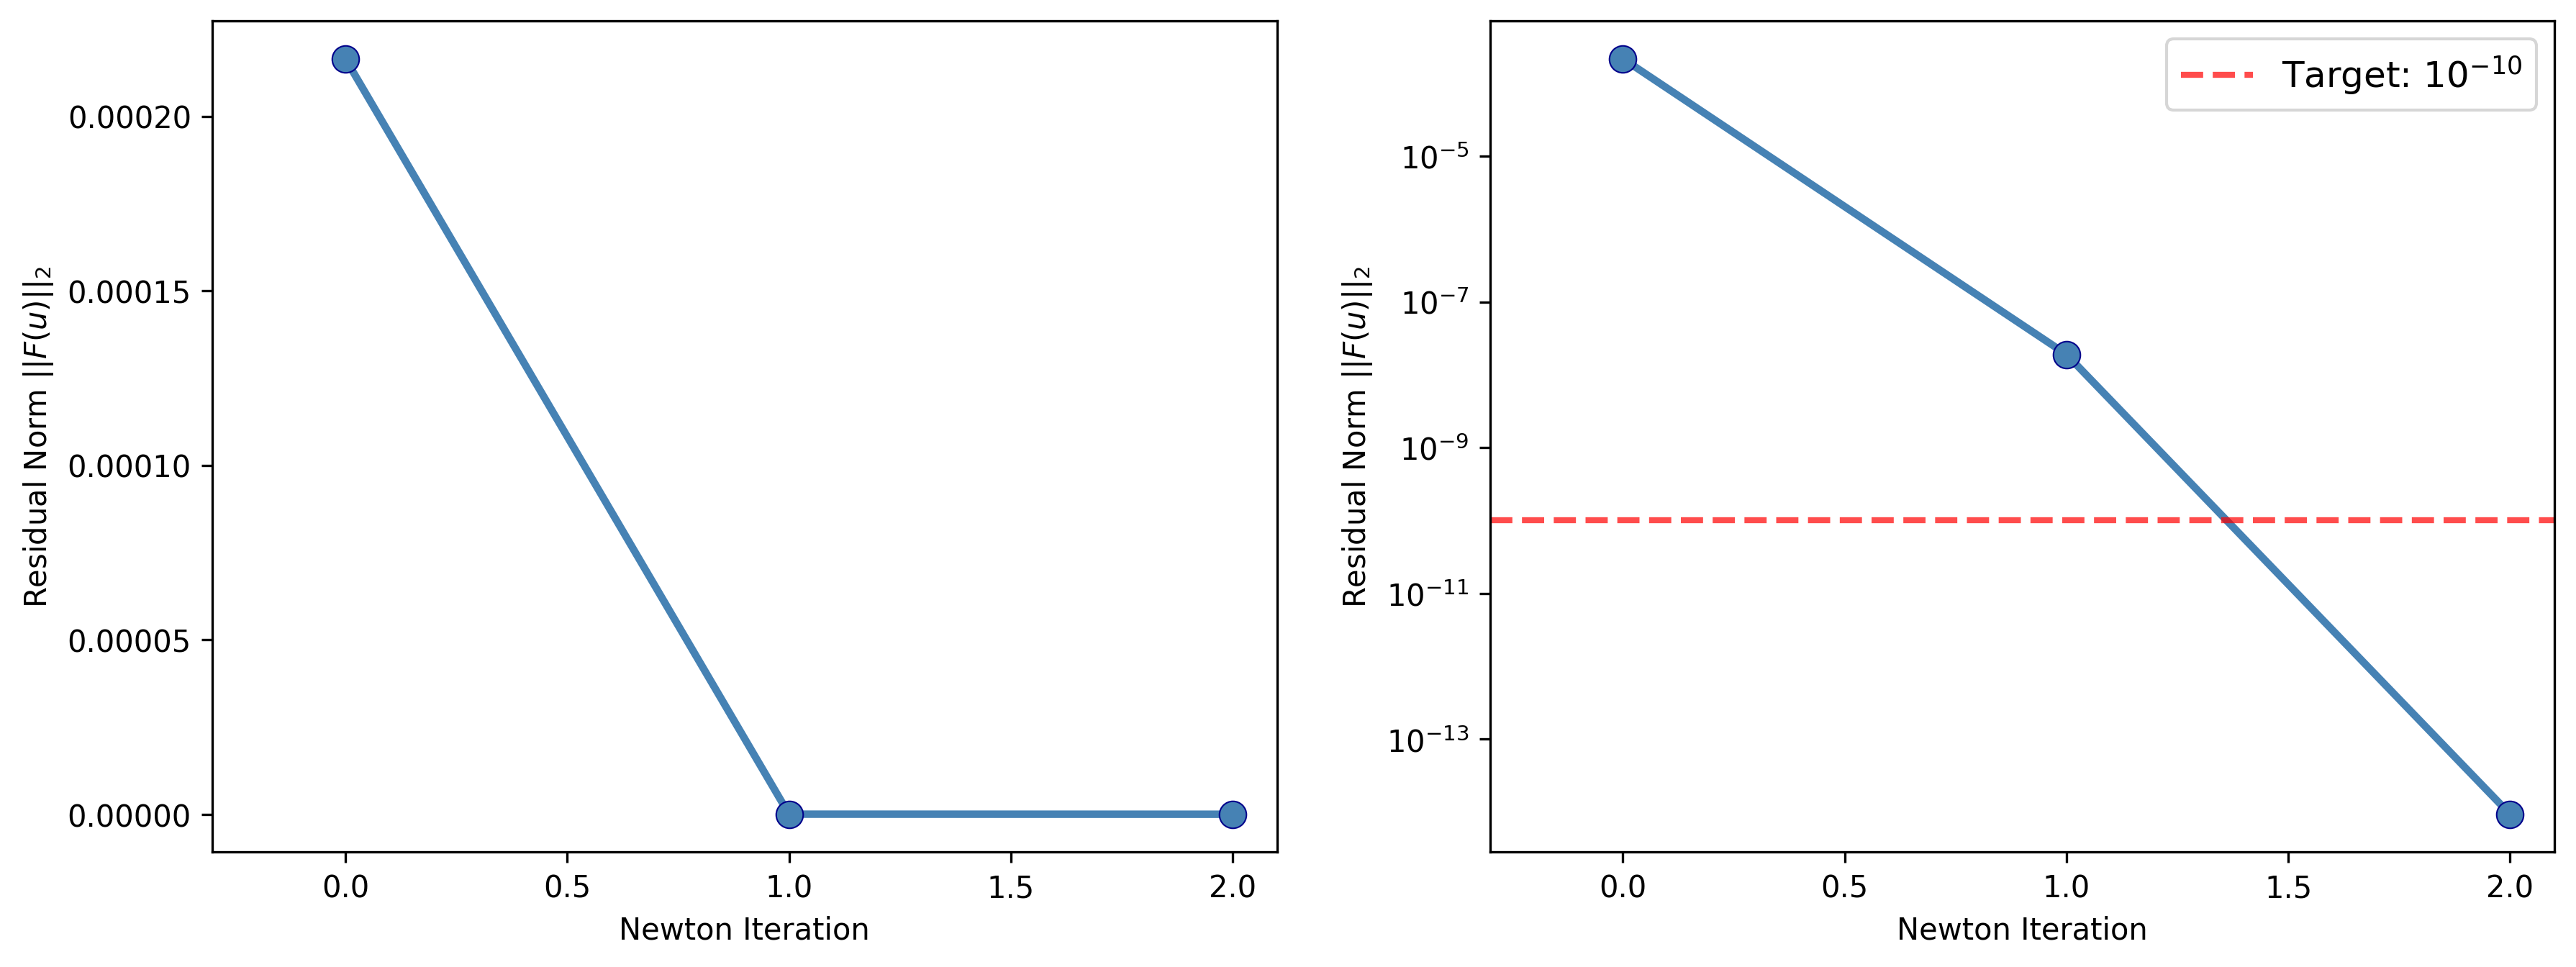
\includegraphics[width=1\textwidth]{../q6_results/convergence_plot.png}
    \caption{Performance and scaling study: nonlinear problem ($\gamma=100$, $p=3$)}
    \label{fig:q6_scaling}
\end{figure}

\section{Question 7}
Rerunning the problem with \texttt{-rct\_linear\_f} (linear RHS: $f = -\nabla^2 u_{\text{exact}}$) 
for both $\gamma = 0$ and $\gamma = 100$ with $p=3$ allows us to isolate the effect of the nonlinear reaction term $\gamma u^p$. Case 1 is linear and uses the equation $-\nabla^2 u = -\nabla^2 u_{\text{exact}}$, which converges in 1 Newton iteration with a relative error of $5.25 \times 10^{-4}$, indicating the solution closely approximates $u_{\text{exact}}$.While the nonlinear onesolves $-\nabla^2 u + 100u^3 = -\nabla^2 u_{\text{exact}}$, requiring 5 Newton iterations and yielding a much larger relative error of $2.03 \times 10^{-1}$, demonstrating that the solution deviates significantly from $u_{\text{exact}}$. The nonlinear reaction term $\gamma u^p = 100u^3$ basically creates a cubic damping effect. Regions where $u$ is large experience stronger  suppression (proportional to $u^3$), resulting in a solution with significantly lower magnitude compared to $u_{\text{exact}}$. The ParaView visualization below
shows that both solutions maintain the Gaussian-like distribution centered at $(0.65, 0.65)$,  but the nonlinear case exhibits substantially reduced amplitude.

\begin{figure}
    \centering
    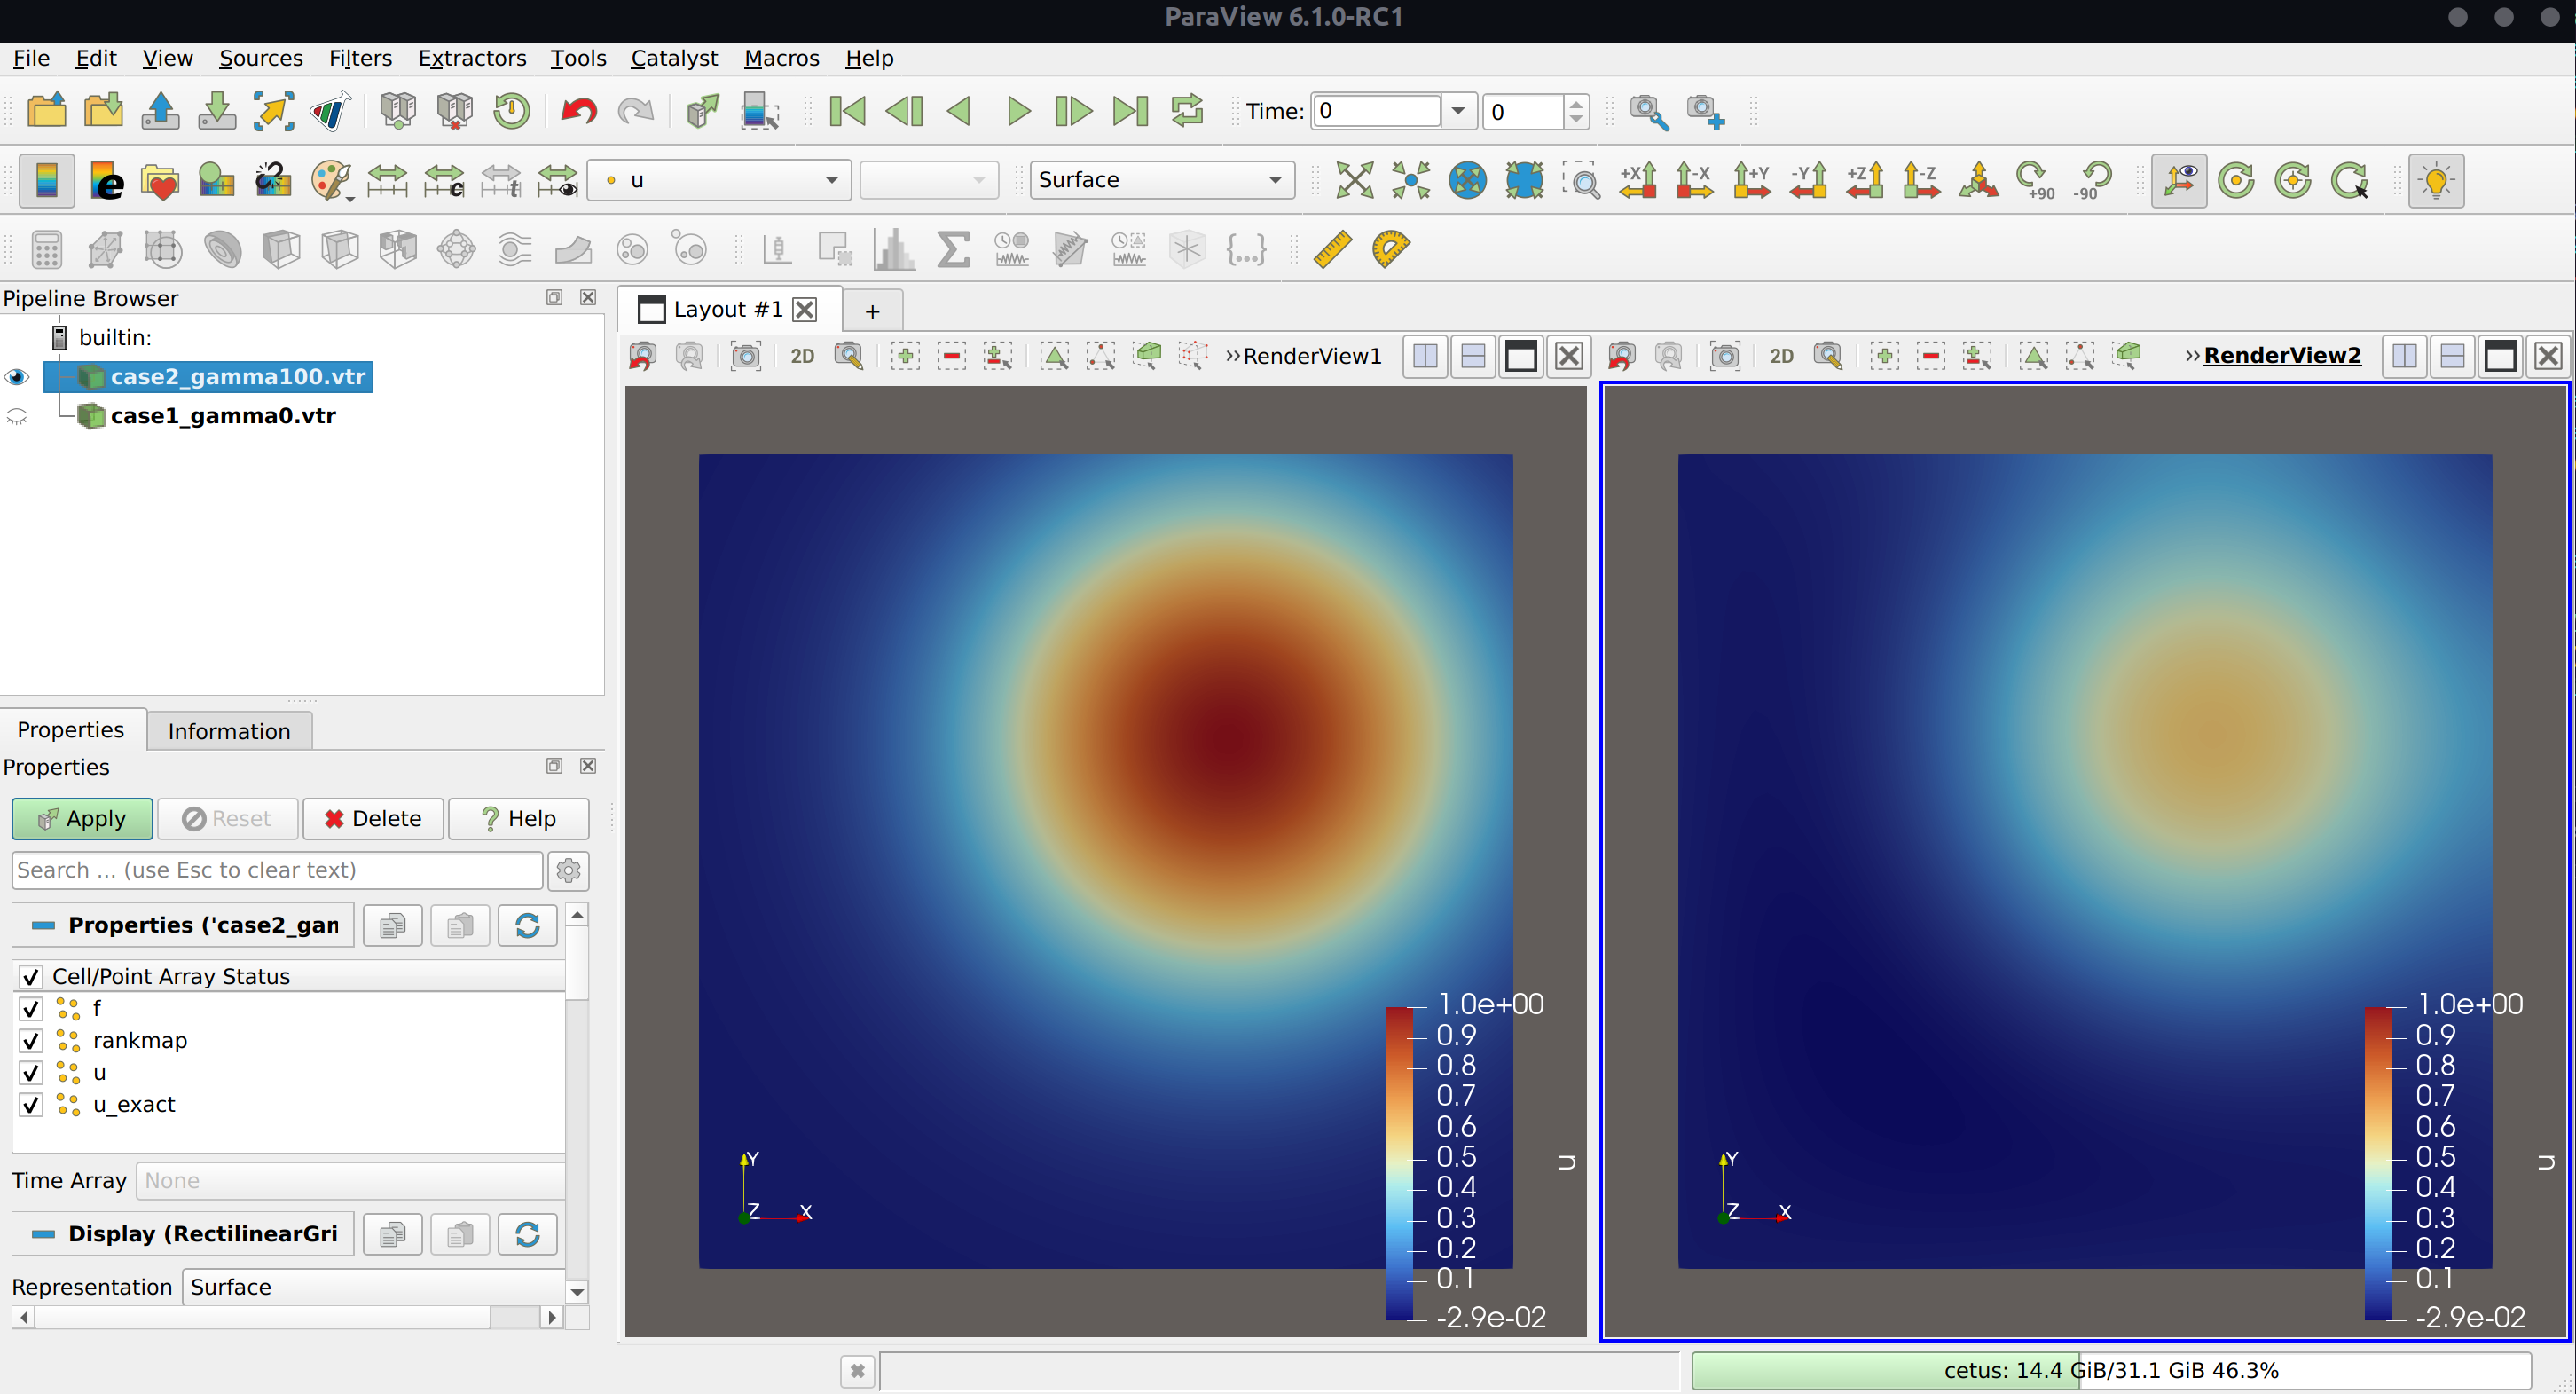
\includegraphics[width=1\textwidth]{../q7_results/gamma000_vs_gamma100.png}
    \caption{Comparison of linear and nonlinear problems ($\gamma=100$, $p=3$), with nonlinear being on the right}
    \label{fig:q7_scaling}
\end{figure}

\newpage
\section{Question 8}
Here we will look at the performance nad scaling for the non-linear problem ($\gamma = 100$, and $p=3$) across different refinements and processors. For that, we make use of \texttt{q8.sh}, which runs the problem for different grid sizes and number of processors. The results are shown in Table \ref{tab:q8_scaling} below and plotted in \ref{fig:q8_scaling}.


The trend for runtime as a function of grid size scales linearly (in log log space) for grid size greater than $65 \times 65$, which is expected for a 2D problem with a direct solver. The speedup relative to the single processor case is sublinear, with the two processor case achieving around 1.5x speedup and the four processor case achieving around 2x speedup for the largest grid size. 

The number of Newton iterations required for convergence remains constant at 3 across all cases, indicating that the nonlinear solver seems robust to changes in grid size and processor count. 

The relative error compared to the exact solution decreases with grid refinement, as expected, with the smallest error achieved on the finest grid. The parallel efficiency decreases with increasing processor count and grid size, indicating sublinear scaling, which is common for parallel solvers due to communication overhead and load imbalance. Note, the definition of this parallel efficiency is relative to the single processor case with grid size $33 \times 33$. Parallelization efficiency drops as we increase the number of processors and grid size, which is expected due to increased communication overhead and load imbalance in larger parallel runs. 
\begin{table}[h]
\centering
\caption{Nonlinear Problem ($\gamma=100$, $p=3$)}
\label{tab:q8_scaling}
\begin{tabular}{cccccc}
\hline
\textbf{Refine} & \textbf{Grid Size} & \textbf{nprocs} & \textbf{Time (s)} & \textbf{Newton Iters} & \textbf{Rel. Error} \\
\hline
2 & $33 \times 33$ & 1 & $1.139 \times 10^{-2}$ & 3 & $8.098 \times 10^{-4}$ \\
2 & $33 \times 33$ & 2 & $1.408 \times 10^{-2}$ & 3 & $8.098 \times 10^{-4}$ \\
2 & $33 \times 33$ & 4 & $2.012 \times 10^{-2}$ & 3 & $8.098 \times 10^{-4}$ \\
\hline
3 & $65 \times 65$ & 1 & $2.223 \times 10^{-2}$ & 3 & $2.025 \times 10^{-4}$ \\
3 & $65 \times 65$ & 2 & $1.842 \times 10^{-2}$ & 3 & $2.025 \times 10^{-4}$ \\
3 & $65 \times 65$ & 4 & $3.648 \times 10^{-2}$ & 3 & $2.025 \times 10^{-4}$ \\
\hline
4 & $129 \times 129$ & 1 & $1.577 \times 10^{-1}$ & 3 & $5.065 \times 10^{-5}$ \\
4 & $129 \times 129$ & 2 & $1.455 \times 10^{-1}$ & 3 & $5.065 \times 10^{-5}$ \\
4 & $129 \times 129$ & 4 & $1.007 \times 10^{-1}$ & 3 & $5.065 \times 10^{-5}$ \\
\hline
5 & $257 \times 257$ & 1 & $7.787 \times 10^{-1}$ & 3 & $1.267 \times 10^{-5}$ \\
5 & $257 \times 257$ & 2 & $5.383 \times 10^{-1}$ & 3 & $1.267 \times 10^{-5}$ \\
5 & $257 \times 257$ & 4 & $4.185 \times 10^{-1}$ & 3 & $1.267 \times 10^{-5}$ \\
\hline
6 & $513 \times 513$ & 1 & $4.188 \times 10^{0}$ & 3 & $3.167 \times 10^{-6}$ \\
6 & $513 \times 513$ & 2 & $2.895 \times 10^{0}$ & 3 & $3.167 \times 10^{-6}$ \\
6 & $513 \times 513$ & 4 & $2.124 \times 10^{0}$ & 3 & $3.167 \times 10^{-6}$ \\
\hline
\end{tabular}
\end{table}


\begin{figure}
    \centering
    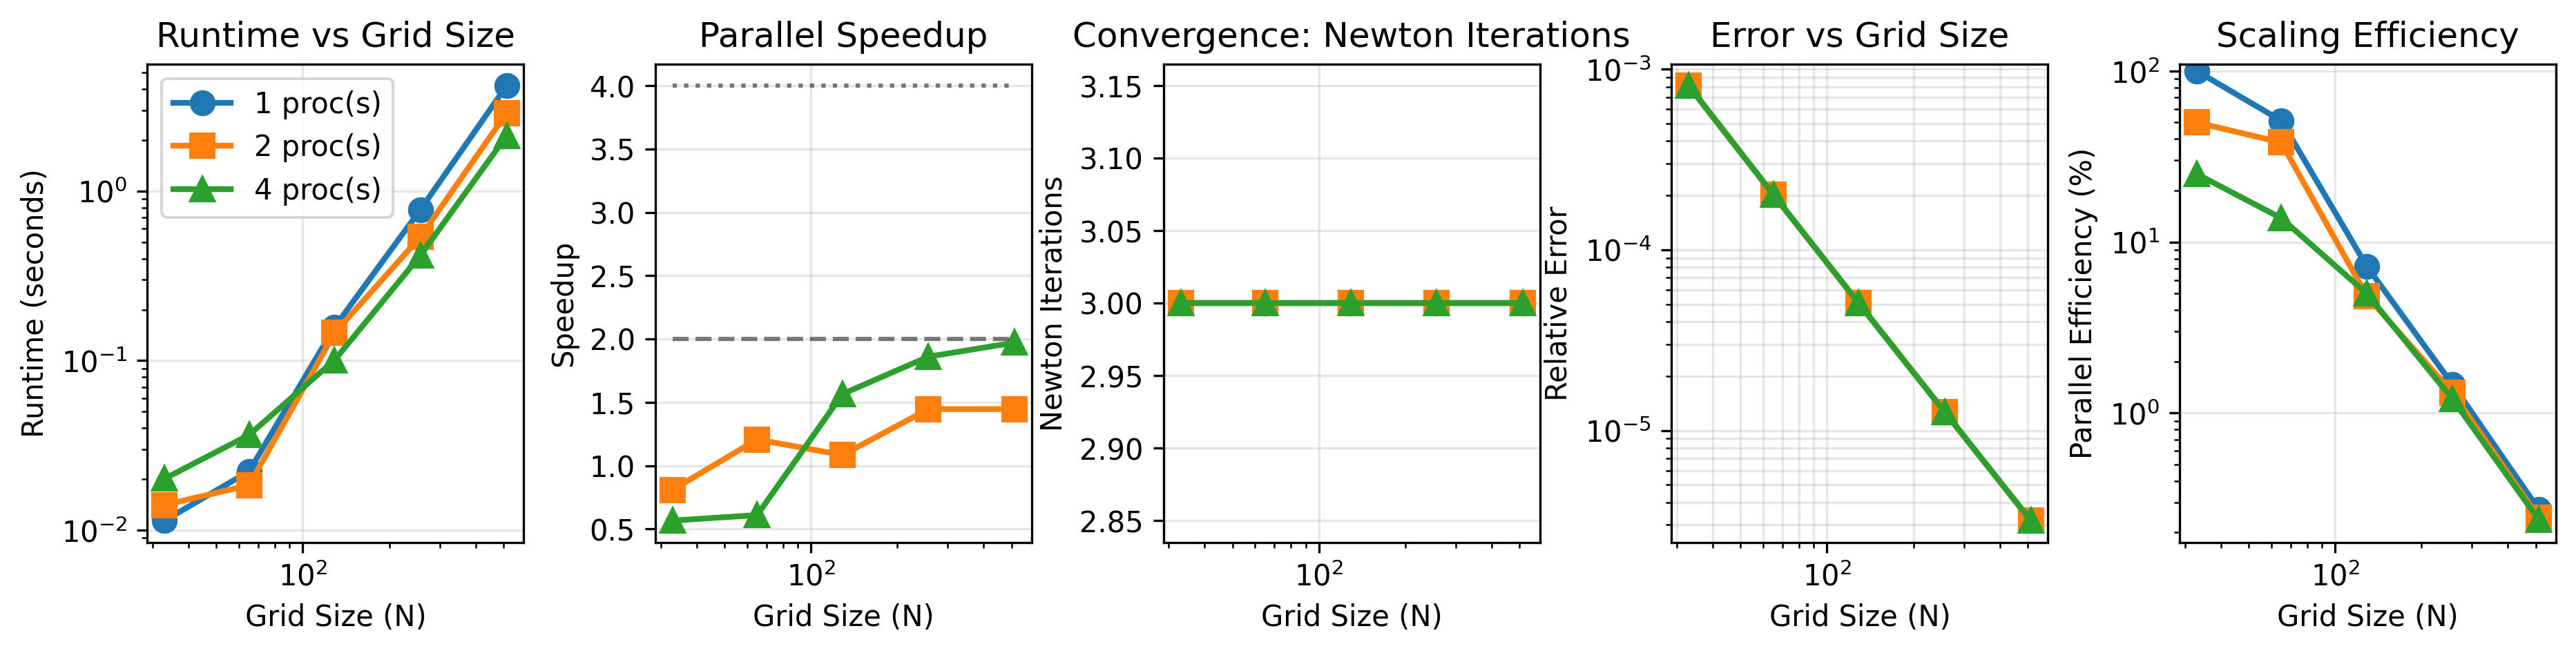
\includegraphics[width=1\textwidth]{../q8_results/scaling_plots.png}
    \caption{Comparison of performance and scaling for the nonlinear problem ($\gamma=100$, $p=3$) across different refinements and processors. The first panel (from left to right) shows the runtime in seconds as a function of grid size for 1 (blue), 2 (orange), and 4 (green) processors. The second panel shows the speedup relative to the single processor case, with ideal linear speedup shown as a dashed and dotted black line for the two and four processors, respectively. The third panel shows the number of Newton iterations required for convergence, which remains constant at 3 across all cases. The fourth panel shows the relative error compared to the exact solution, which decreases with grid refinement. The fifth panel shows the parallel efficiency as a percentage, which decreases with increasing processor count and grid size, indicating sublinear scaling.}
    \label{fig:q8_scaling}
\end{figure}





\end{document}